\documentclass[12pt]{article}
%\documentclass{amsart}

%\renewcommand{\baselinestretch}{2}

\usepackage{datetime}
\usepackage{graphicx}
\DeclareGraphicsExtensions{.pdf}


\title{{\Large University of Bath Mechanical Engineering Department 
Technical Report 13/05:}\\~\\{\LARGE A new fractal curve}}

\author{Adrian Bowyer\\
\\
{\em http://adrianbowyer.com}}


\newdate{date}{06}{09}{2005}
\date{\displaydate{date}}


\begin{document}
 
\input{epsf}
 
\maketitle
 
\begin{abstract}

\noindent
The new fractal curve described in this report is deterministic
(though it appears at a casual glance to be random), simple to
specify, and easy and quick to compute.  It will automatically fill
any pre-defined bounded and connected region of the plane, is
self-avoiding, and never self-intersects.  The definition of the curve
is given, along with pictures of it in two dimensions generated by a
C++ implementation (this software will be freely available on the web
on the publication of this work in the reviewed literature).
Simulations of the curve are statistically analysed with the result
that---under a well-defined and broad range of conditions---its
fractal dimension is about 1.5.  The curve can use a single line
segment inside the bounded region as a starting pattern, or a
non-self-intersecting polyline.  Several of the curves can be
generated in the same region, and will fill it without crossing
themselves or each other.  The definition extends to any number of
dimensions; in {\em K} dimensions the curve would become a {\em K-1}
dimensional hypersurface filling a bounded hypervolume.

\vspace{3mm}
                                                             
\noindent
{\em Keywords:} Peano curve, Hilbert curve, Sierpinski gasket, Koch
curve, coastline curve, fractal, space-filling curve.

\end{abstract}

 
\section*{Introduction}

A common computational way of generating an approximation to a random
fractal curve (similar to the coastlines discussed by Mandelbrot
\cite{mandelbrot}) is to bisect a straight line segment and to move
the half-way point at right angles to the segment by some (pseudo-)
random distance.  This process is then repeated recursively on the two
halves thus created, with the expected distance of the random movement
reduced by a fixed factor (say 0.5) at each level of the recursion.
Figure \ref{r-frac} from the Boston Center for Polymer Studies
\cite{boston-cps} shows the result of such a process.

\begin{figure}[h!]
 \begin{center} 
  \resizebox{0.4 \textwidth}{!}{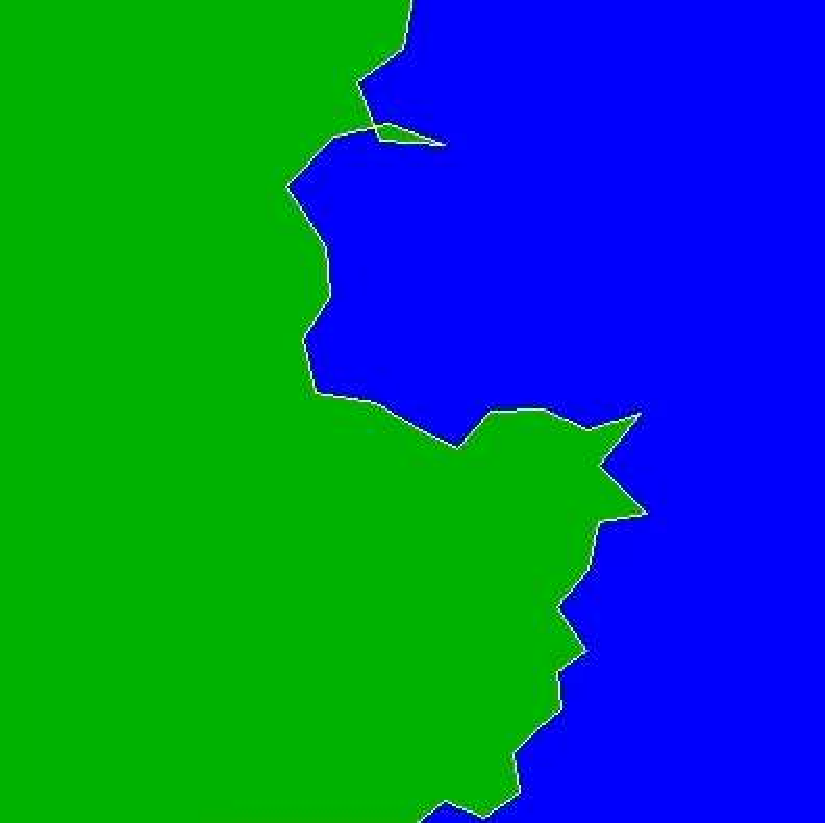
\includegraphics{Pix/r-frac}}
  \parbox{110mm}{\caption{\label{r-frac} The first five stages of
      recursion of a random fractal curve from the Boston Center for
      Polymer Studies \cite{boston-cps}.  Note the self-intersection
      near the top.}}
\end{center}
\end{figure}

The method just outlined produces a curve, but that curve is not
guaranteed to reside in any particular region of the plane, and nor is
it guaranteed never to self-intersect.  

Regular space-filling curves such as the Peano \cite{peano-orig} and
Hilbert \cite{hilbert-orig} curves (Figure \ref{hilbert}(a)) never
self-intersect, of course, and---if the recursion is
infinite---completely cover a known rectangular region of the plane,
which is to say that their fractal dimension \cite{mb2} is 2.  There
are variations on them which will fill non-rectangular regions as well
as rectangular ones (see Figure \ref{hilbert}(b)).  The region they
fill, however, is entirely decided by their elemental shape and the
recursion rule.

A self-avoiding curve should also never self-intersect.  Peitgen,
J\"{u}rgens and Saupe \cite{peitgen} describe a self-avoiding
space-filling curve, but this will again only fill a rectangular
region.  It also prompts the authors to say, ``With a plain `multiple
reduction copy machine'\footnote{This is an explicatory thought
machine (by analogy with a thought experiment) of the authors for
producing multiple copies of a shape under transformations.} it is not
possible to create a self-avoiding and space-filling curve that is
aesthetically pleasing.''

\begin{figure}[h!]

 \begin{center} 
  \resizebox{0.4 \textwidth}{!}{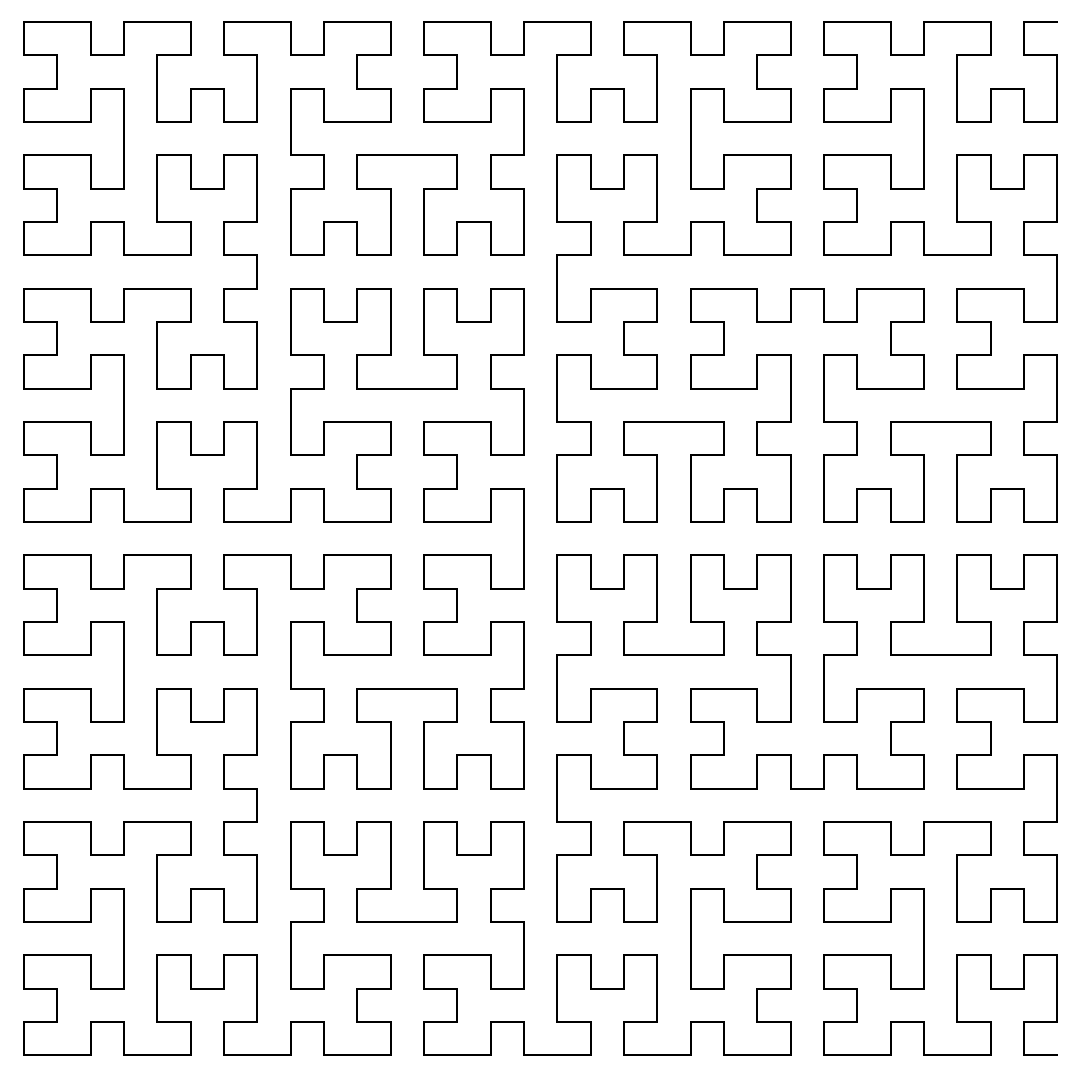
\includegraphics{Pix/hilbert}}
  \resizebox{0.4 \textwidth}{!}{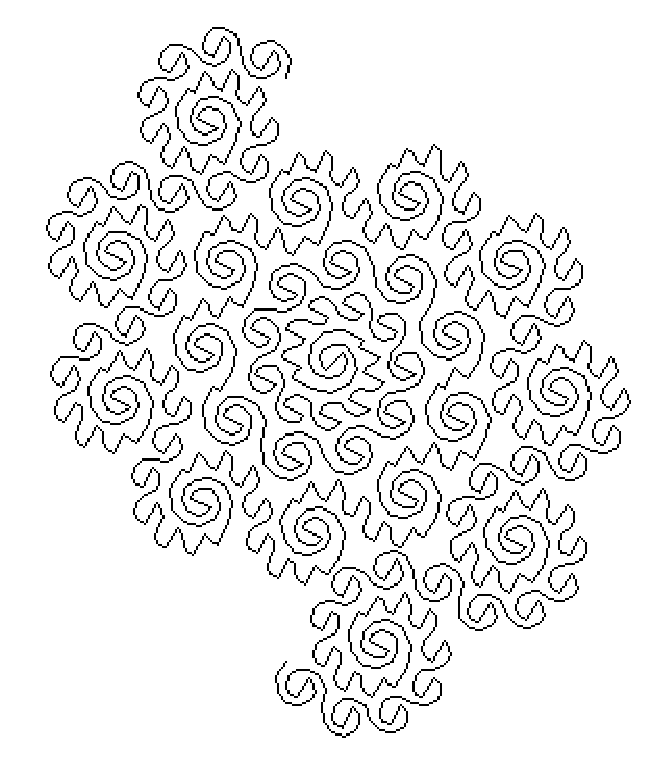
\includegraphics{Pix/bendy}}
  \parbox{110mm}{\caption{\label{hilbert} (a)The first five stages of
  recursion of a Hilbert curve \cite{hilbert-orig} from Balayoghan
  \cite{texas-hilbert}. (b) A regular space-filling curve filling a
  non-rectangular region.}}
\end{center}
\end{figure}

The recursive curve described in this report is self-avoiding, and is
also deterministic like a Peano curve, in that its shape is entirely
decided by its initial conditions.  But it does not consist of
multiple scaled copies of a fixed initial shape (that is, it is not a
product of one of Peitgen, J\"{u}rgens and Saupe's multiple
reduction copy machines).  And I contend that it is aesthetically
pleasing\footnote{Here the reader must make appropriate allowances for
authorial bias.}.

It also has the useful properties that it will fill any pre-defined
connected area of the plane and will never
self-intersect\footnote{These two properties were the initial
requirements that I had for the curve.  They came from a number of
engineering applications that were the genesis of it.}.  It is
possible to generate it starting from any given non-self-intersecting
polyline within the area (including a single line
segment).  The new curve is also quick and simple to compute.

Though this is not investigated here, the definition of the curve
extends quite straightforwardly and comprehensively to form
(hyper)surfaces in any number of dimensions.

This report is intended to be a descriptive and empirical introduction
to the new curve as others may also have applications for it.  Should
the reader wish to follow this up, I have made C++ software for
generating examples of the curve freely available under the GNU Public
Licence \cite{gpl} from Github at
https://github.com/AdrianBowyer/fractal.  

The reader wishing to find good books on fractals and space-filling
curves is referred to the ones by Hans Sagan \cite{sagan} and Kenneth
Falconer \cite{falconer}.

\section*{The new curve}

Consider the following method of generating a curve, this time within
a bounded area: bisect a straight line segment that lies completely
within the area and move the half-way point along the bisector (as in
the coastline curve described at the start of the Introduction).  But
this time move the point {\em as far as possible as long as it stays
at least some exclusion radius away from every other part of the curve
and the boundary.}  `As far as possible' here means that both halves
of the bisector either side of the initial segment need to be
considered.  The point chosen is the one that lies farthest along the
bisector in either direction away from the initial segment.

Now repeat that process recursively on the two halves, reducing the
value of the exclusion radius by some factor at each recursive step,
again as before.  In general the exclusion is for all parts of the
curve except the split-line-segment's two immediately-joining
before-and-after line segments, as its distance to them must always be
zero.

The result is a curve such as the one shown in Figure \ref{new_f1}, which was
generated by the C++ program mentioned above.
\begin{figure}[h!]
 \begin{center} 
  \resizebox{0.4 \textwidth}{!}{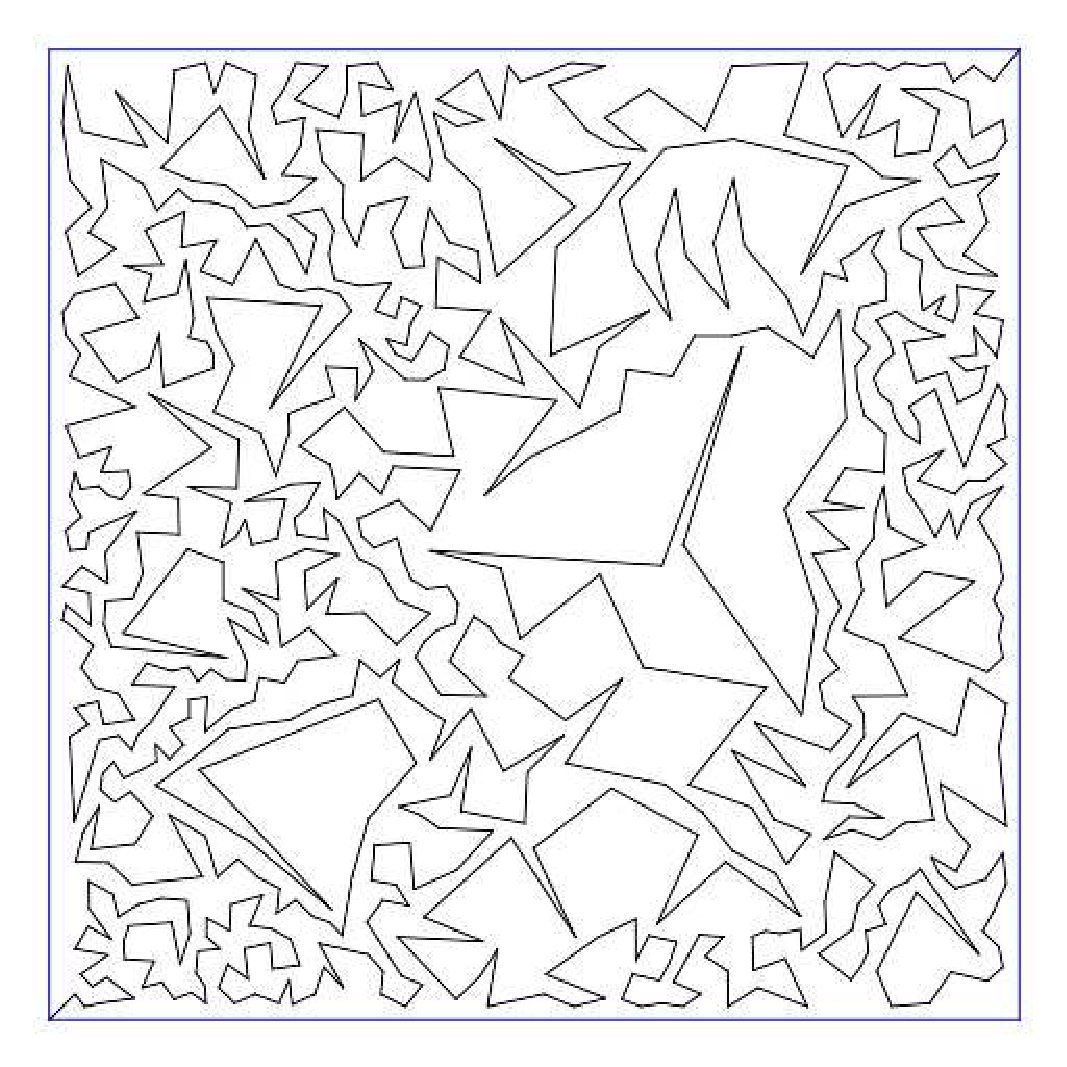
\includegraphics{Pix/new_f1}}
  \parbox{110mm}{\caption{\label{new_f1} An example of the new curve.  The closed
  area was the unit square, and the starting line segment was its
  diagonal from the origin.  The initial exclusion radius was 0.1, and
  this was reduced by a factor of 0.8 at each level of recursion.  The
  recursion was run 10 times.}}
\end{center}
\end{figure}

\section*{Characteristics of the new curve}

\begin{figure}[h!]
 \begin{center} 
  \resizebox{0.3 \textwidth}{!}{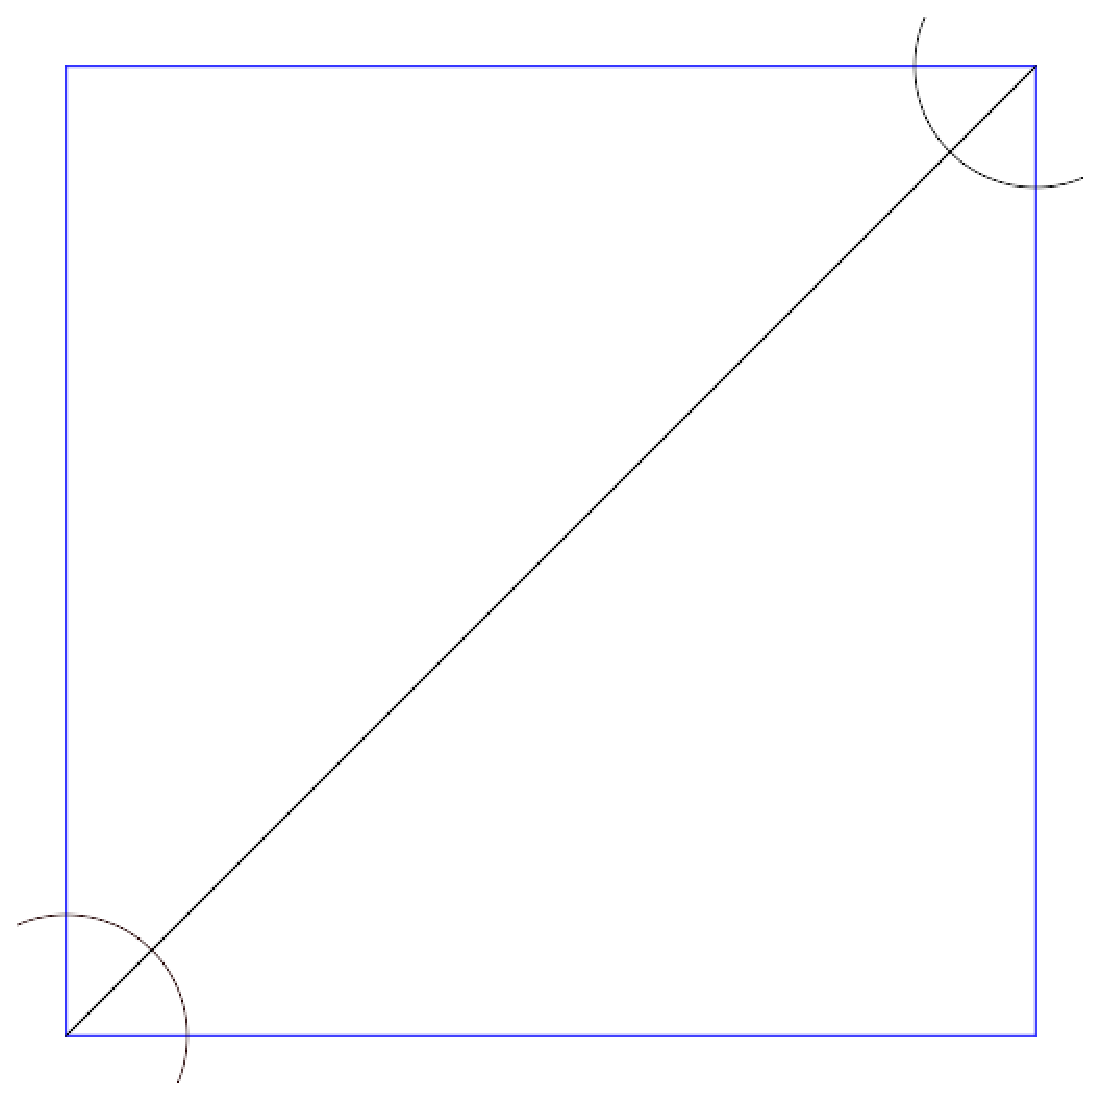
\includegraphics{Pix/sequence1}}
  \resizebox{0.3 \textwidth}{!}{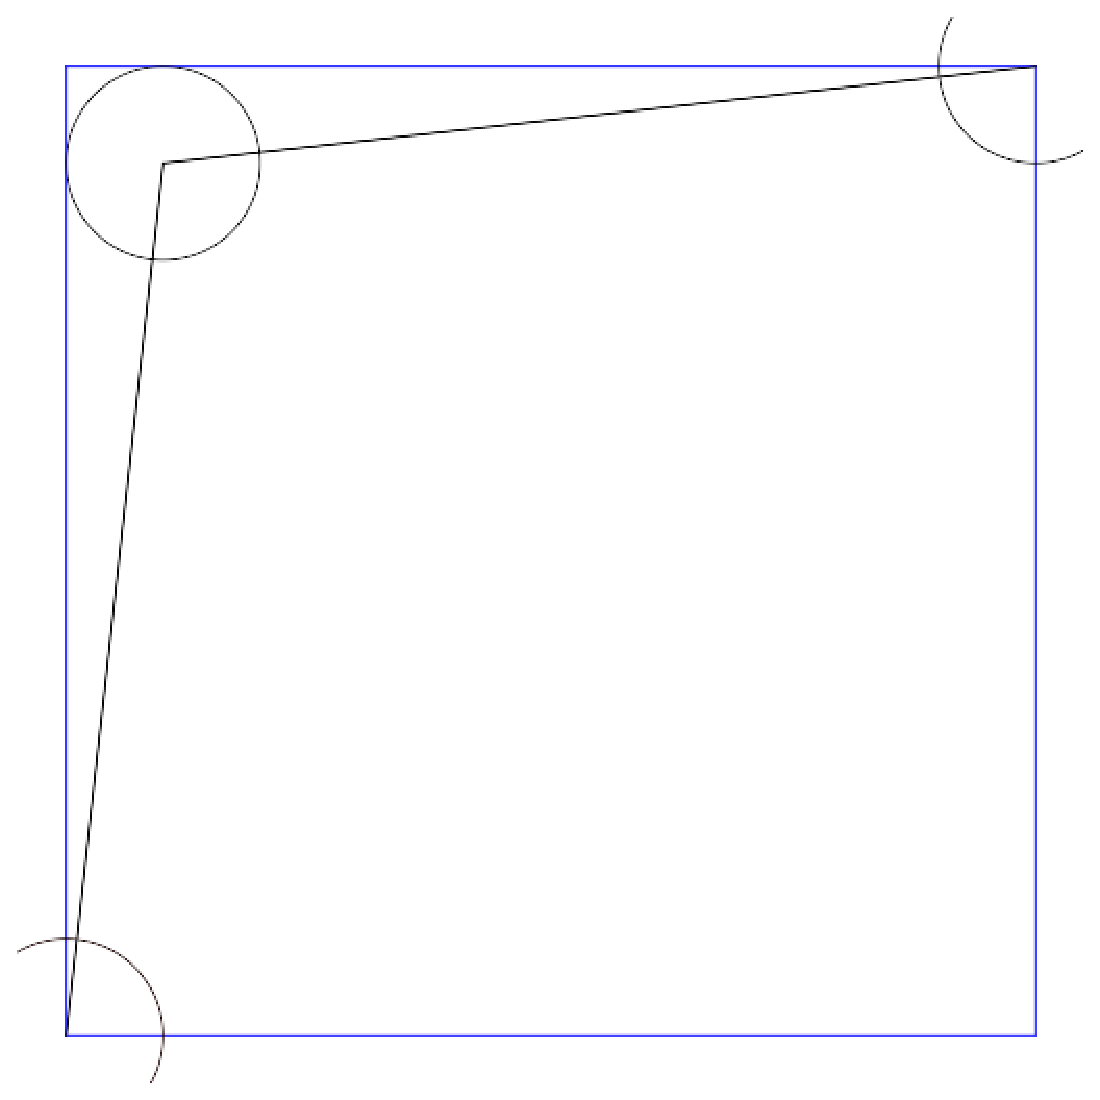
\includegraphics{Pix/sequence2}}
  \resizebox{0.3 \textwidth}{!}{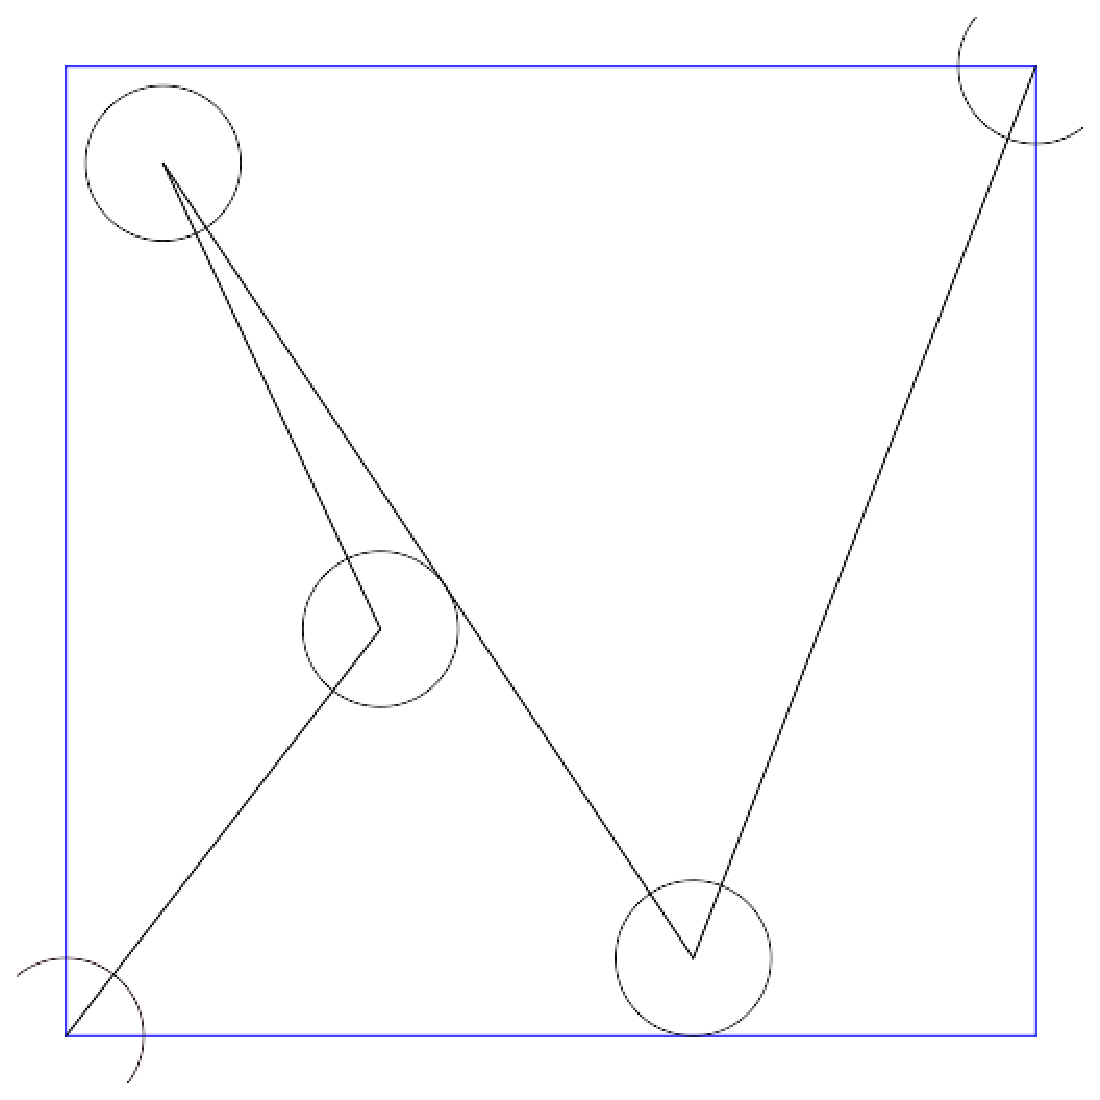
\includegraphics{Pix/sequence3}}\\
  \resizebox{0.3 \textwidth}{!}{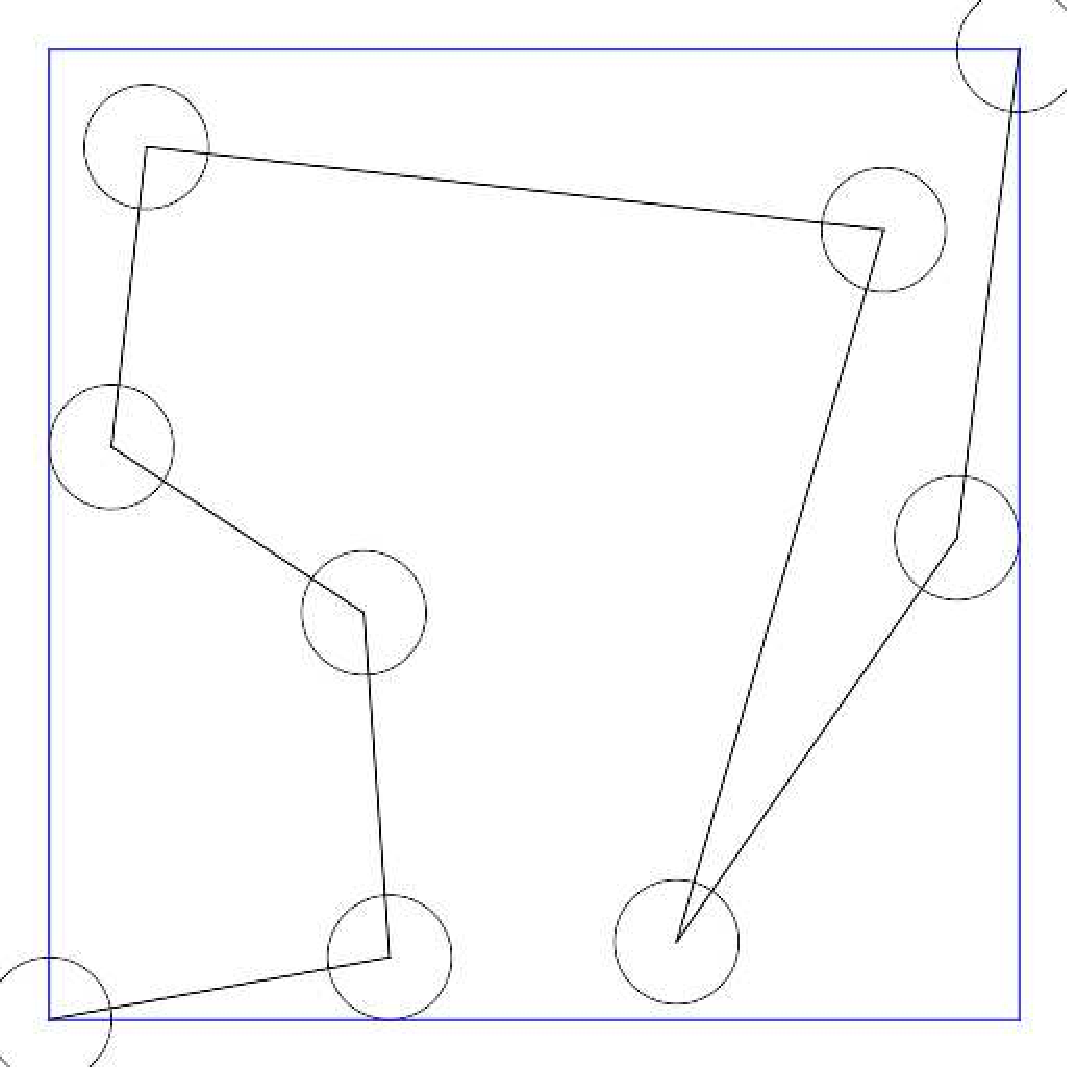
\includegraphics{Pix/sequence4}}
  \resizebox{0.3 \textwidth}{!}{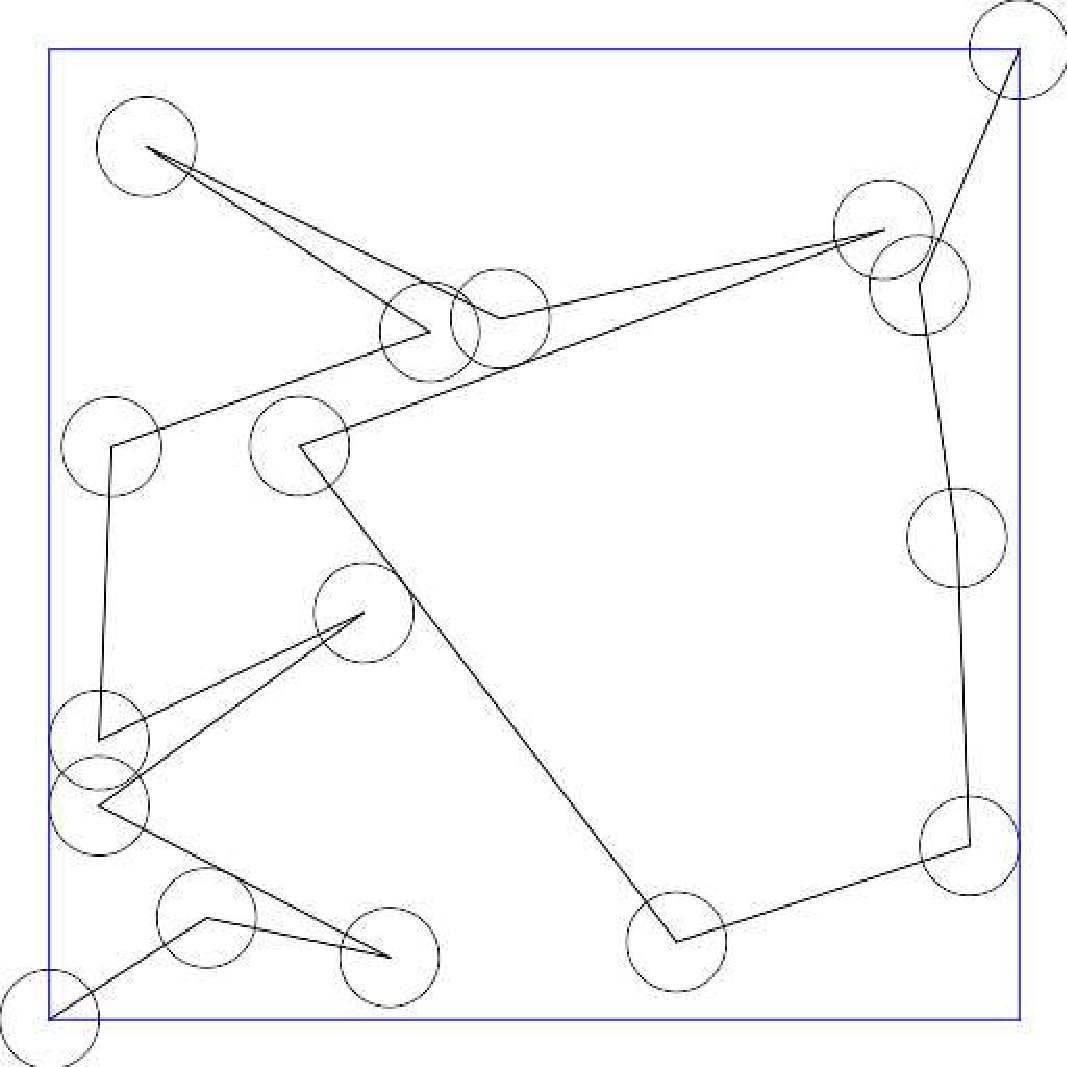
\includegraphics{Pix/sequence5}}
  \resizebox{0.3 \textwidth}{!}{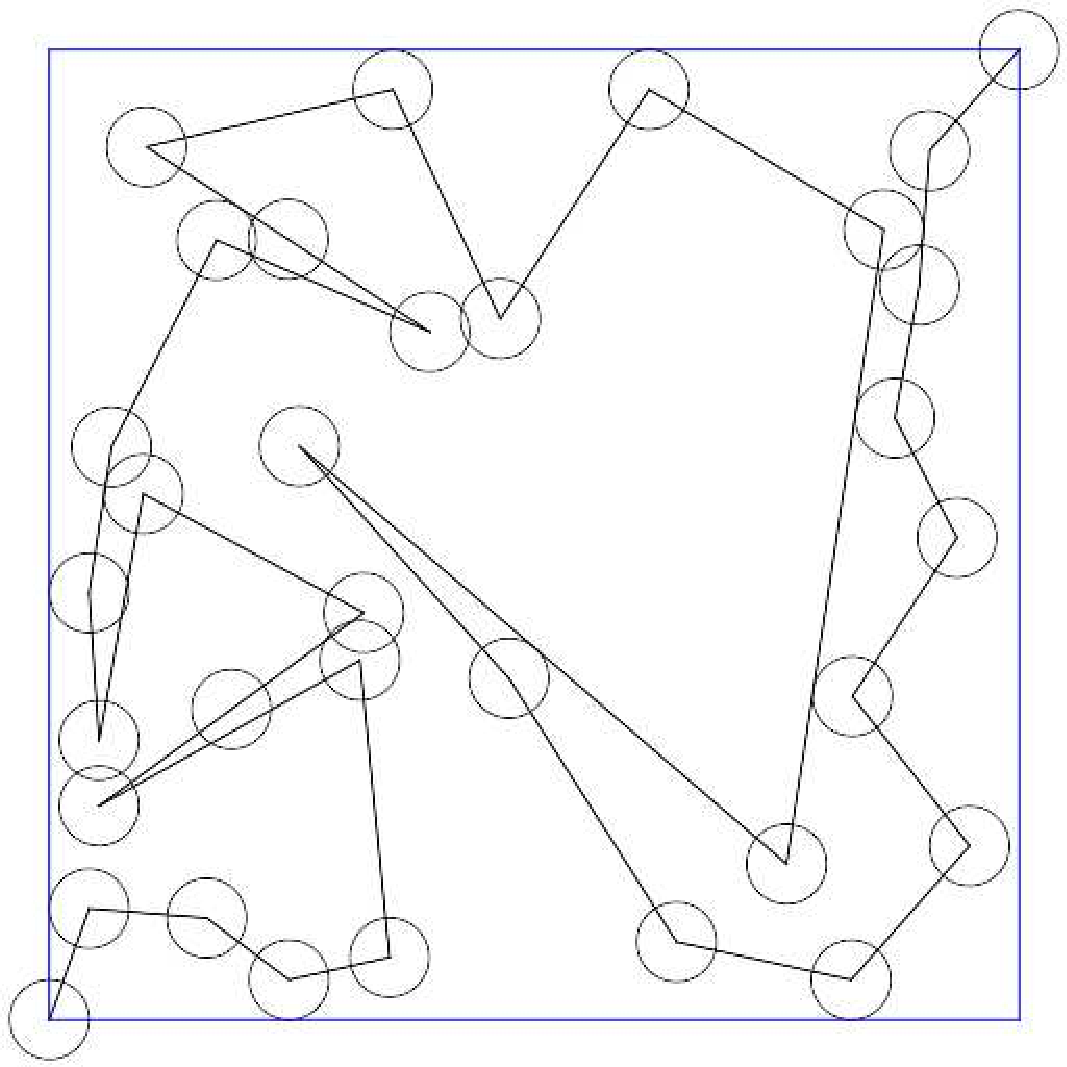
\includegraphics{Pix/sequence6}}
  \parbox{110mm}{\caption{\label{sequence} The original segment and the first five
  recursions of the curve in Figure \ref{new_f1}.  The recursion was
  done breadth-first, and the polyline being generated was alternately
  scanned from bottom left to top right and then back again. The discs are
  the exclusion radii at each recursion level.}}
\end{center}
\end{figure}

Figure \ref{sequence} shows the original square diagonal and the first
five recursions in the generation of the curve in Figure \ref{new_f1}.
Clearly the order in which the recursion is done will affect the
resulting curve.  This example used breadth-first recursion, and the
curve was alternately scanned from bottom left to top right, and then
back again.  If the example in Figure \ref{new_f1} is computed
breadth-first, but always scanned from bottom left to top right then
the result is as in Figure \ref{oneway}.  
\begin{figure}[h!]
 \begin{center} 
  \resizebox{0.4 \textwidth}{!}{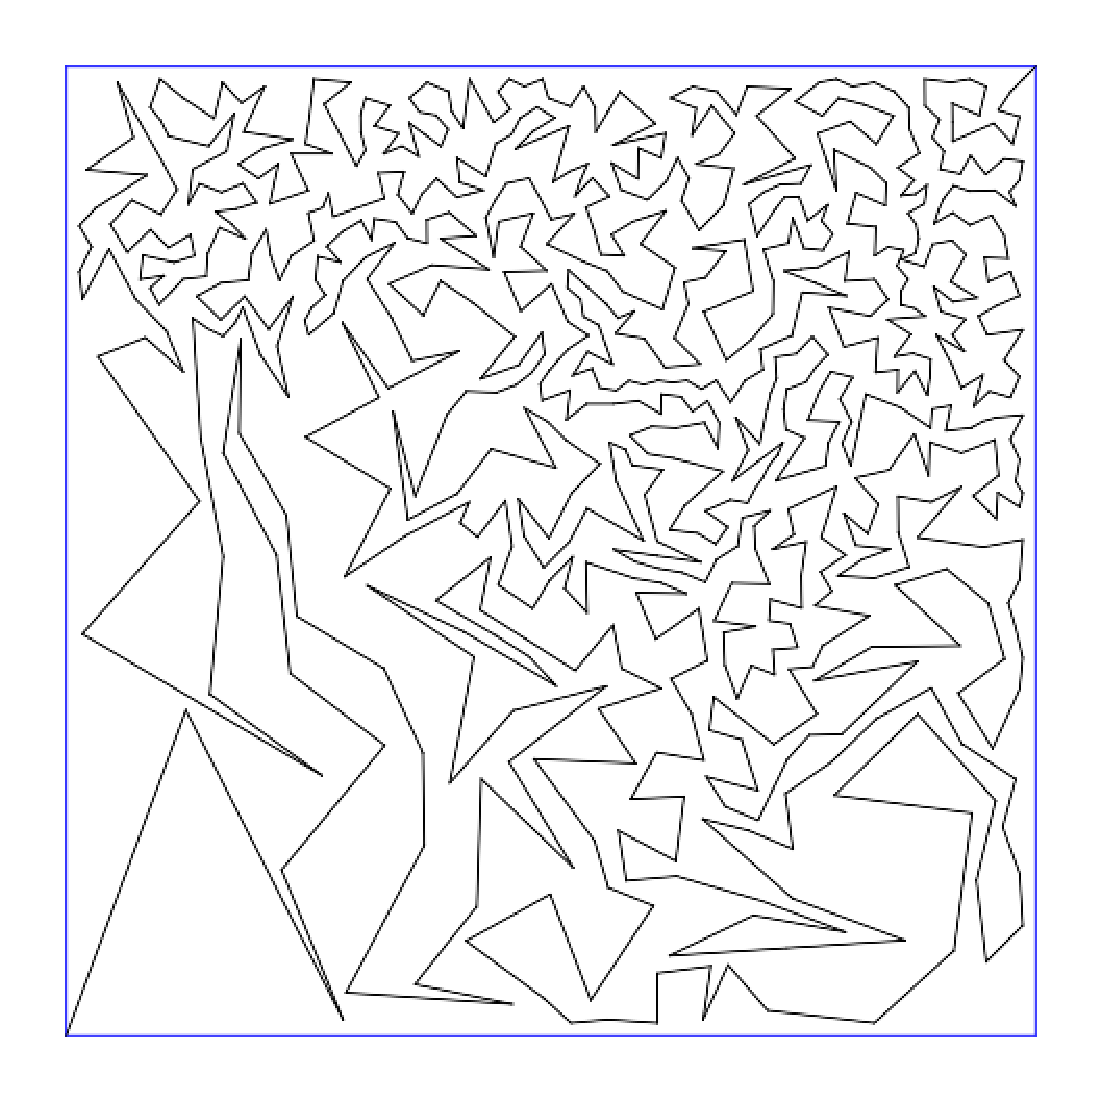
\includegraphics{Pix/new_f2}}
  \parbox{110mm}{\caption{\label{oneway} The same conditions as Figure
  \ref{new_f1}, except that the curve was always scanned from bottom
  left to top right.}}
\end{center}
\end{figure}
Note how this has led to large line segments near the origin and
smaller ones near the top right.  More on this below.  If the
recursion were to be done depth-first this would generate a much
greater bias, as, after the first division, the first half of the
original line would be fully divided before the second half was
considered as anything more than an obstruction.  The choice of
recursion sequence is one of the freedoms available in the definition
of the curve.

The first division in Figure \ref{sequence} obviously involves a
degenerate choice between two possibilities in that---because of
symmetry---the split-point could equally have been moved to the
bottom-right corner of the square.  Note that, even though the result
of that first division is almost as symmetrical, the second division
is completely determined by the order in which the segments of the
polyline were visited.  Other than such degeneracies (which in general
will almost-surely never happen), the curve is completely determined
by the starting conditions, the recursion sequence, and the factor by
which the exclusion radius is reduced at each step.

\begin{figure}[h!]
 \begin{center} 
  \resizebox{0.4 \textwidth}{!}{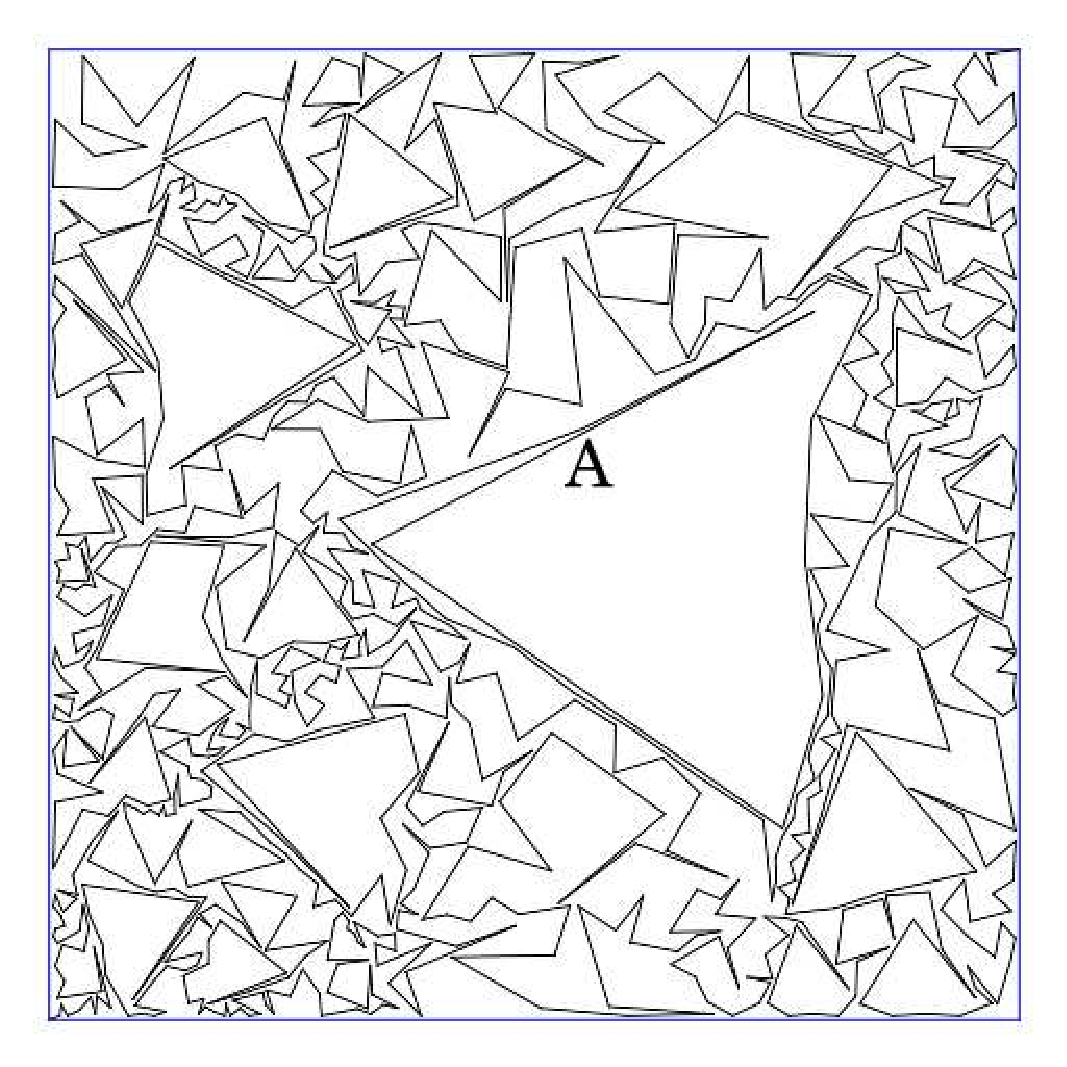
\includegraphics{Pix/new_f07a}}
  \resizebox{0.4 \textwidth}{!}{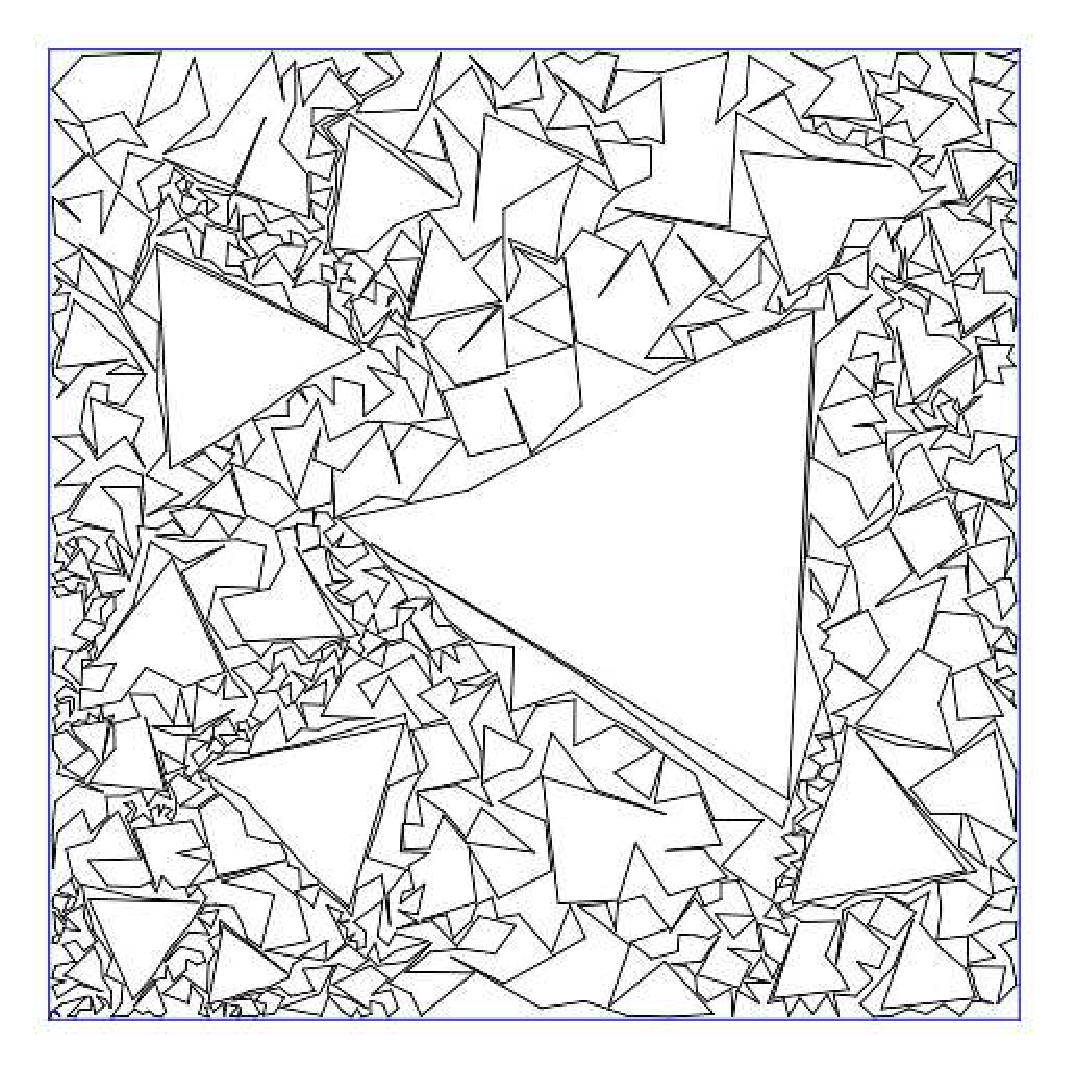
\includegraphics{Pix/new_f07b}}
  \parbox{110mm}{\caption{\label{new_f07} (a) The same conditions as Figure
  \ref{new_f1}, except that the exclusion radius reduction factor was
  0.7 instead of 0.8. (b) The next level of recursion down, in which
  the line segment labelled A has been split and the split point moved
  to near the opposite vertex of the triangle-shaped void.}}
\end{center}
\end{figure}

Two other freedoms available in the definition of the curve are the
choice of that initial exclusion radius and its reduction factor.
Figure \ref{new_f07} (a) shows the curve resulting from the same
conditions as Figure \ref{new_f1}, but with a reduction factor of 0.7
instead of 0.8.

The `gaps' in the pattern (more pronounced in Figure \ref{new_f07}
than in Figure \ref{new_f1}) are filled by subsequent recursions as
illustrated by Figure \ref{new_f07} (b), where the line segment
labelled A in the left-hand figure has split with the resulting point
moving across the triangle-shaped void to near the opposing vertex.
This gives rise to an interesting phenomenon: the stability of
near-equilateral-triangle-shaped voids in patterns with
low values of the exclusion-radius reduction-factor.  When such a
shape arises, the stability happens because one of its edges gets
split and the split point moves to near the opposite vertex, roughly
preserving the shape.  This is illustrated in Figure \ref{triang},
which shows the first few stages of recursion on an actual equilateral
triangle inside a slightly larger equilateral boundary.

\begin{figure}[h!]
 \begin{center} 
  \resizebox{0.3 \textwidth}{!}{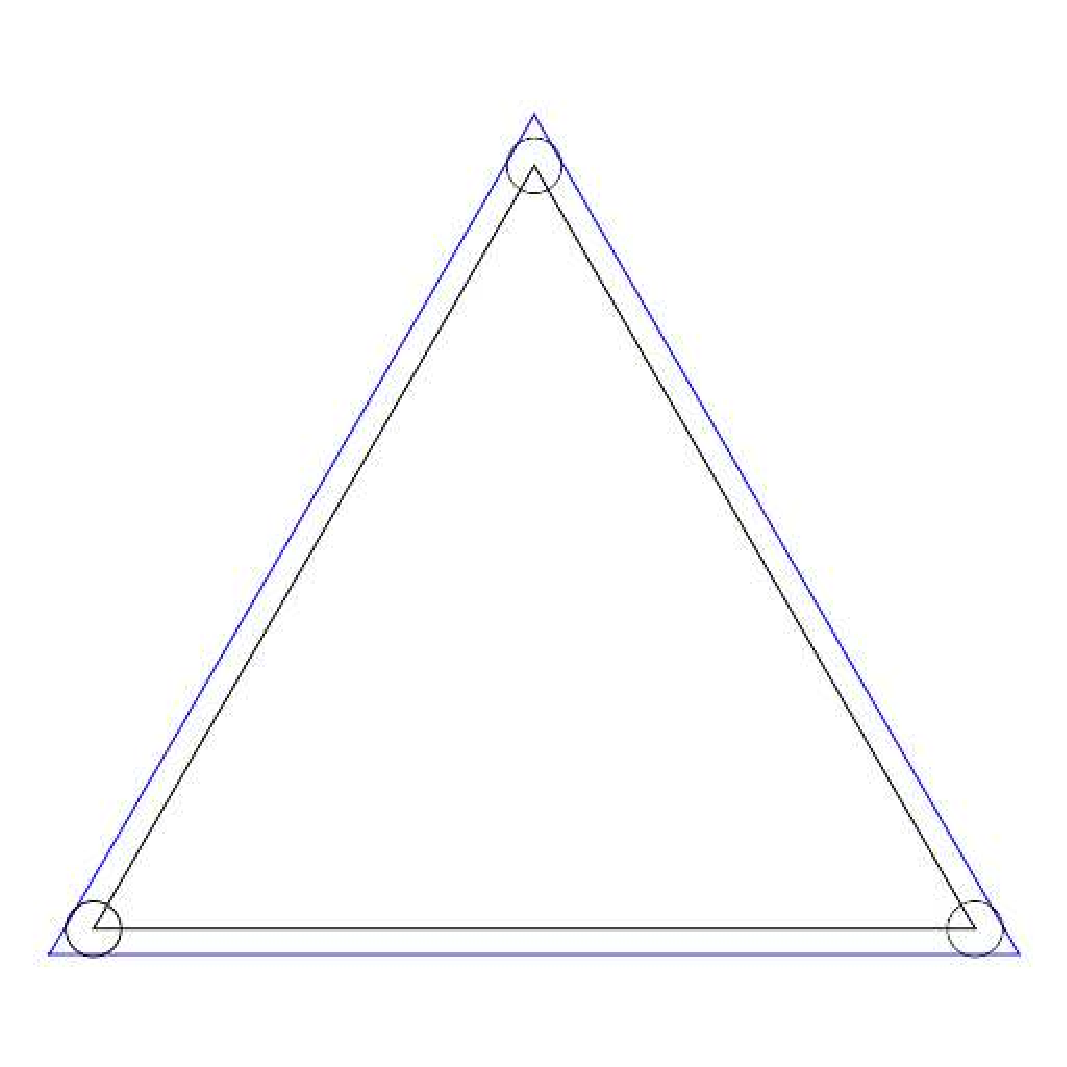
\includegraphics{Pix/triang0}}
  \resizebox{0.3 \textwidth}{!}{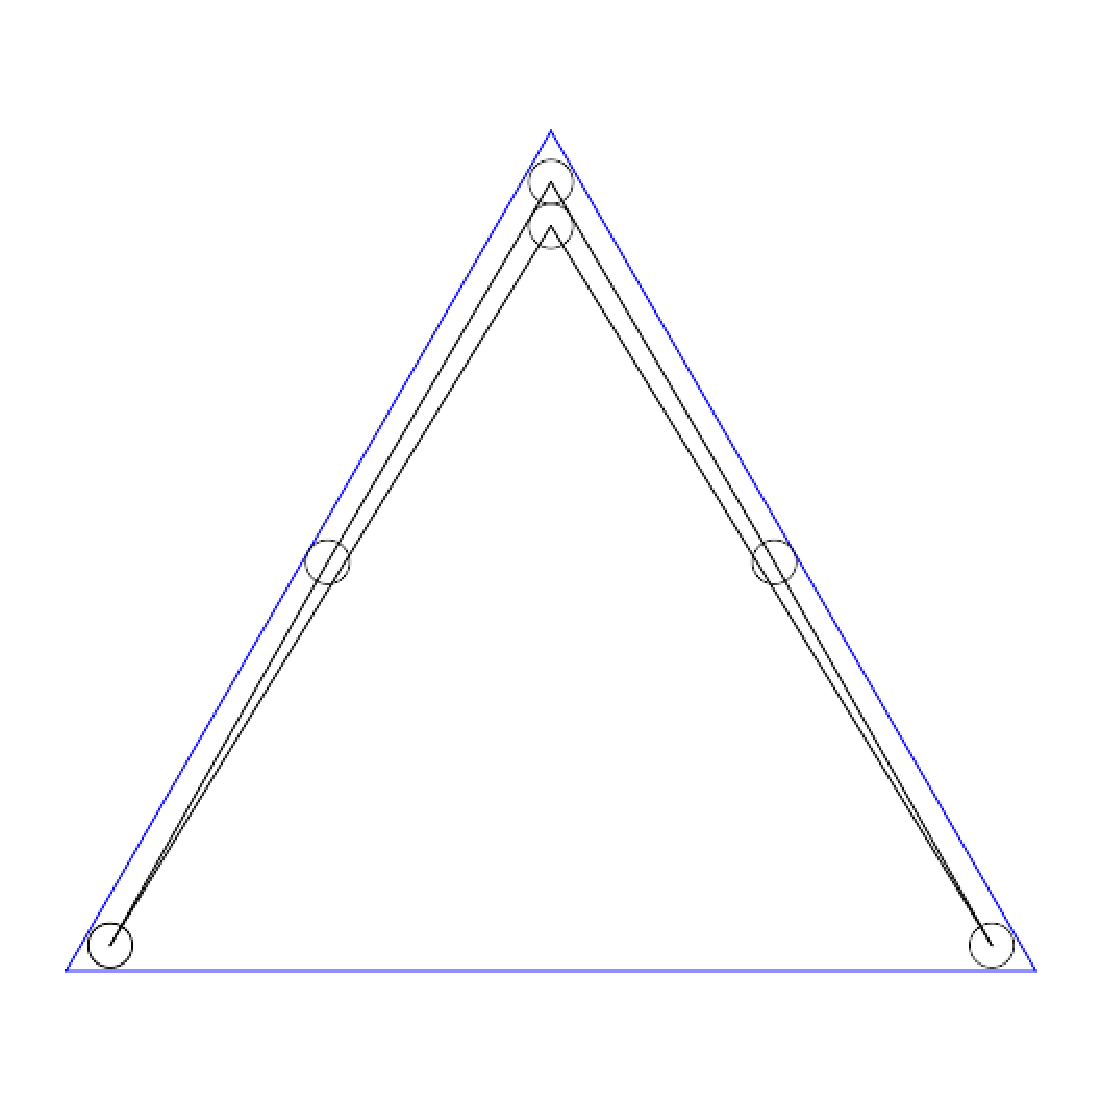
\includegraphics{Pix/triang1}}
  \resizebox{0.3 \textwidth}{!}{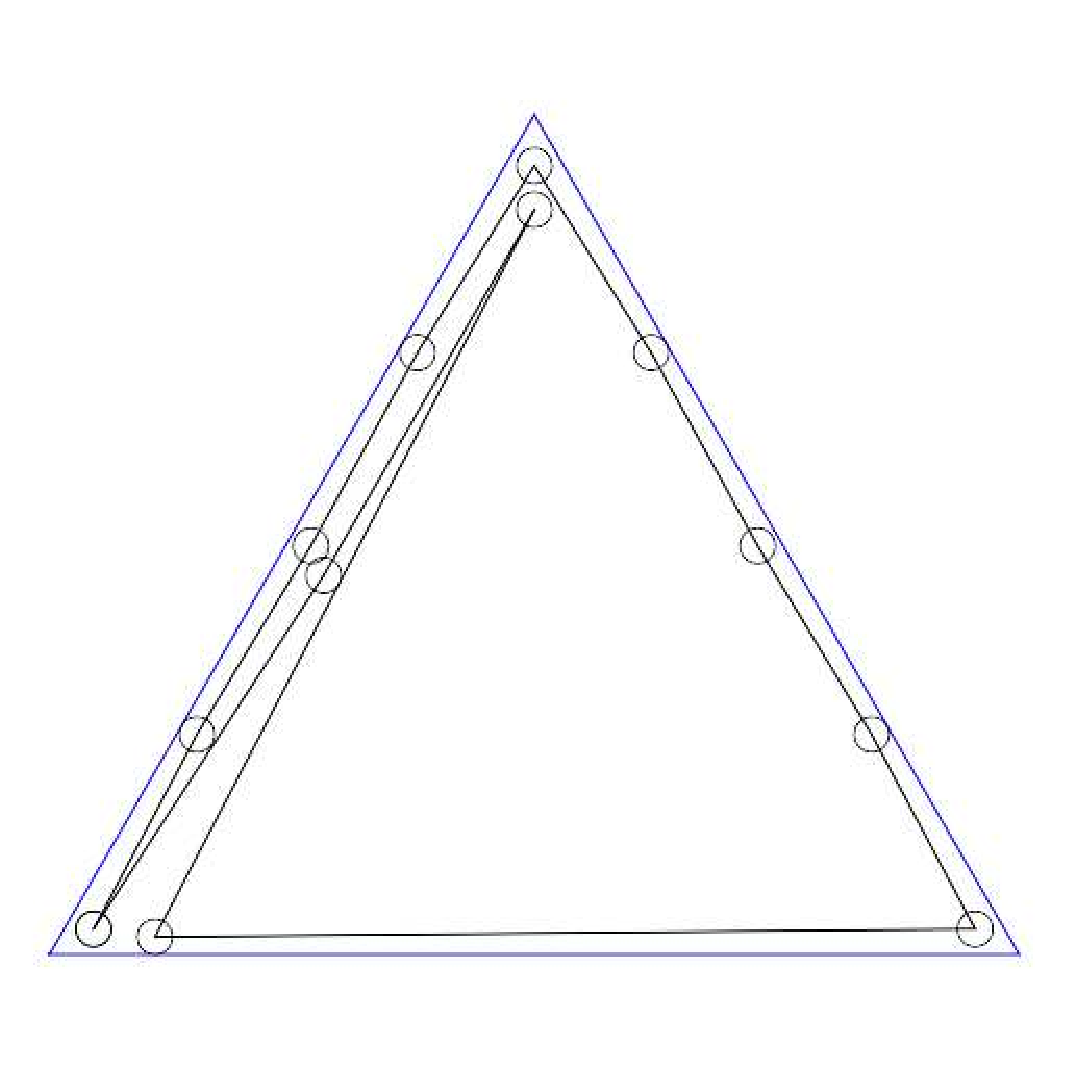
\includegraphics{Pix/triang2}}\\
  \resizebox{0.3 \textwidth}{!}{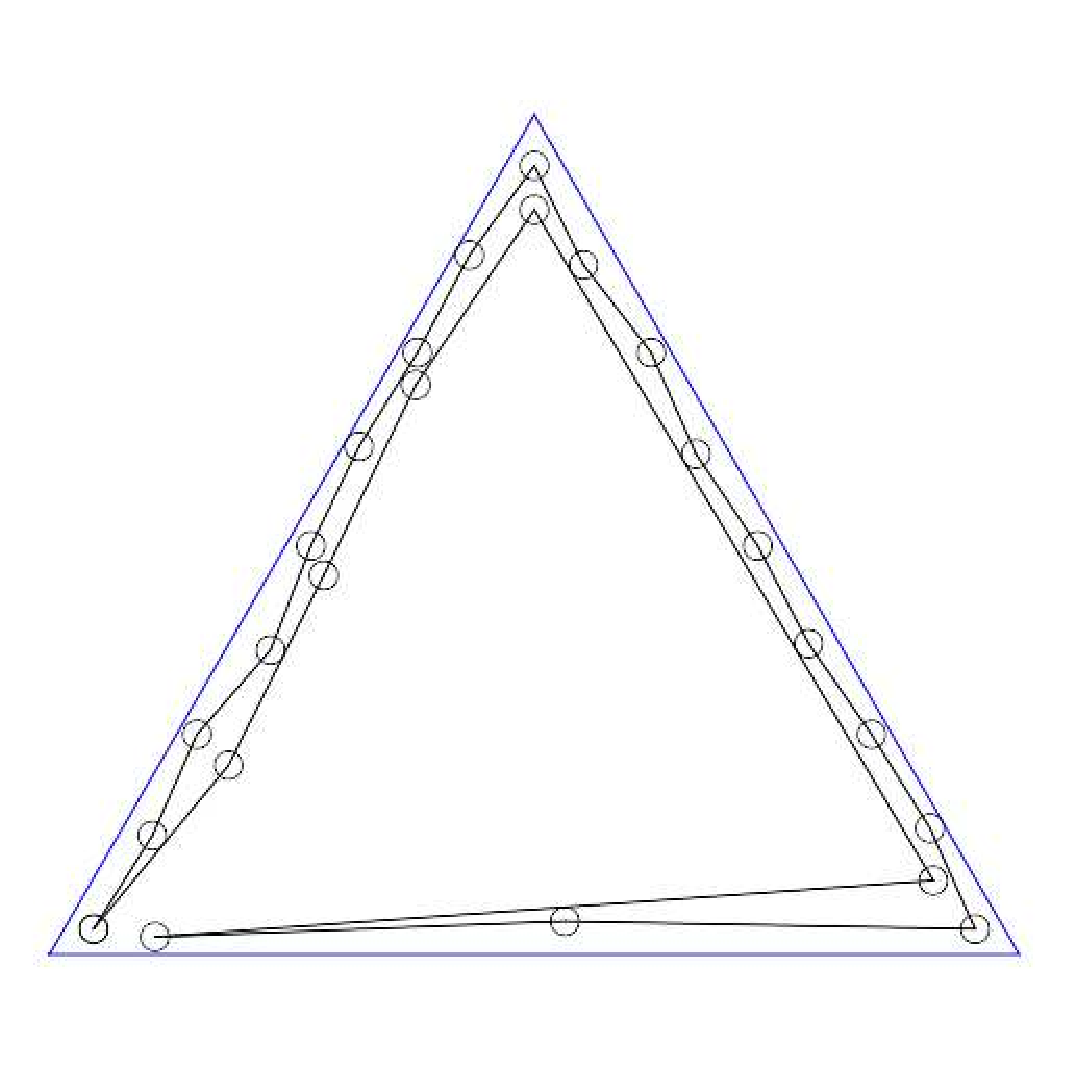
\includegraphics{Pix/triang3}}
  \resizebox{0.3 \textwidth}{!}{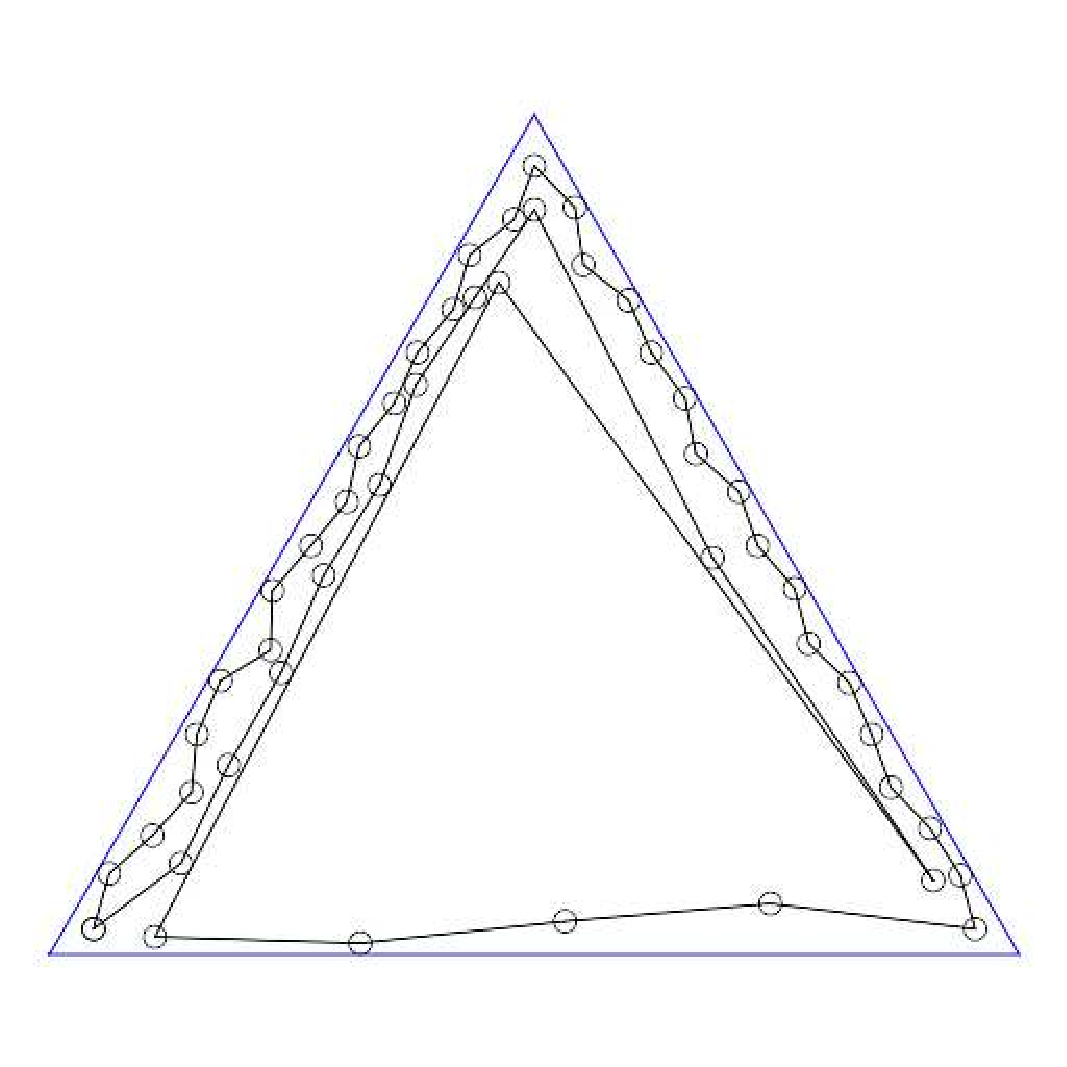
\includegraphics{Pix/triang4}}
  \resizebox{0.3 \textwidth}{!}{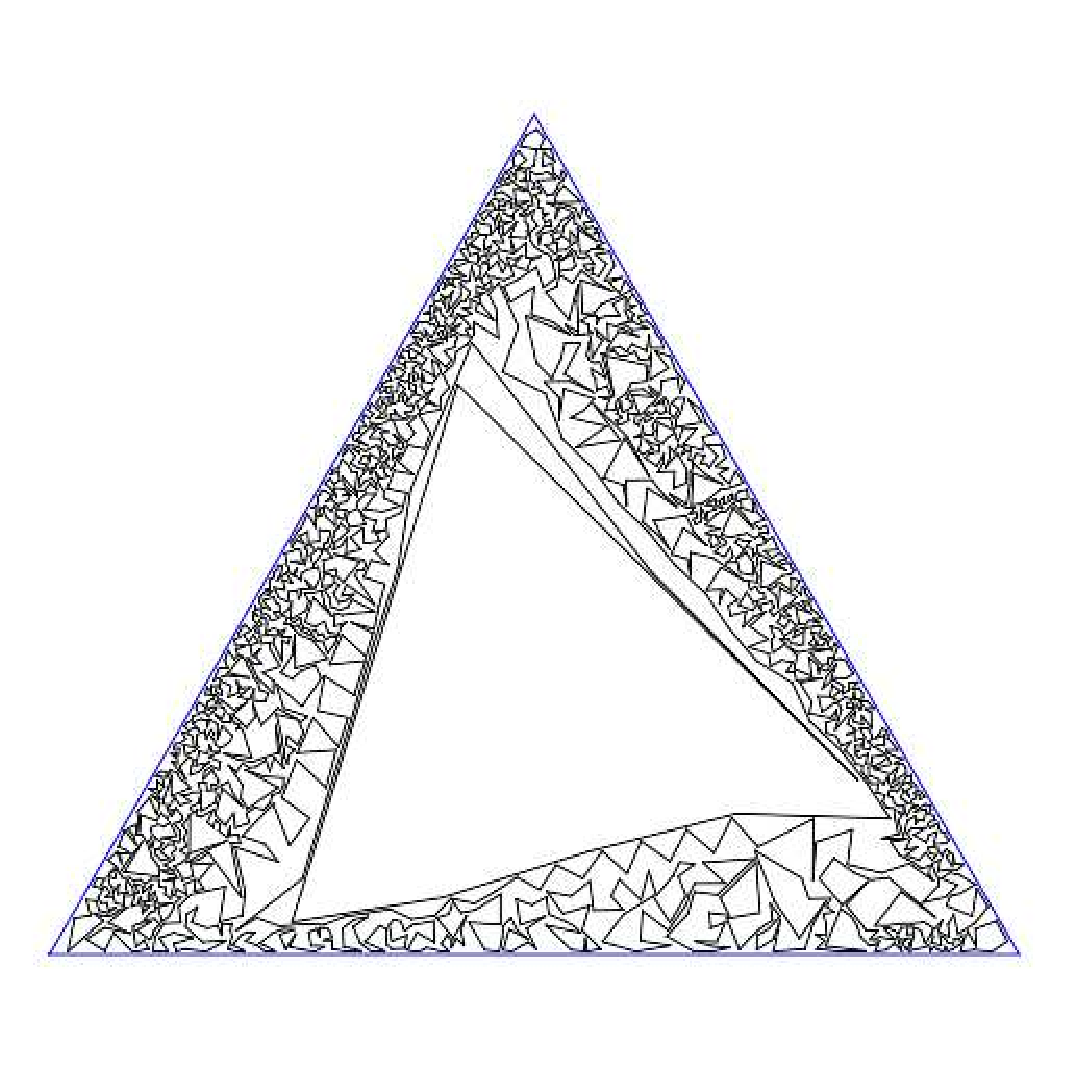
\includegraphics{Pix/triang10}}
  \parbox{110mm}{\caption{\label{triang} The stability of an
  equilateral triangle: the starting configuration, the first four
  recursions, and the tenth recursion.}}
\end{center}
\end{figure}

High values of the reduction factor avoid this phenomenon for
intuitively obvious reasons: the segments are being split and becoming
shorter and shorter, but the exclusion radius is not falling so fast
with the recursion.  The curve therefore is becoming more flexible and
string-like (as opposed to being like a chain of hinged rods),
and its freedom of movement is constrained by the comparatively high
exclusion radius values---it threads its way between other parts of
itself near to the median boundaries defined by the exclusion discs.

\section*{Simulation and statistics}

If the curve were a true fractal, one would expect its length to
increase with the depth of recursion as a power law, which is to say
that one would expect

$$
\ln (L) = d \ln (\frac{2^N}{L_0})
$$

\noindent
where $L$ is a measured length of the curve, $L_0$ is the length of
the original line that was split to make the curve, $N$ is the depth
of recursion ($N = 0$ at $L = L_0$), and $d$ is the power-law
exponent.  The value of $\frac{2^N}{L_0}$ is the number of times the
first segment has been cut divided by its original length.  In other
words, it is an inverse resolution-length for the total length
measurement.  The fractal dimension of the curve, $D$, would be given
by $D = d + 1$.

\begin{figure}[h!]
 \begin{center} 
  \resizebox{0.8 \textwidth}{!}{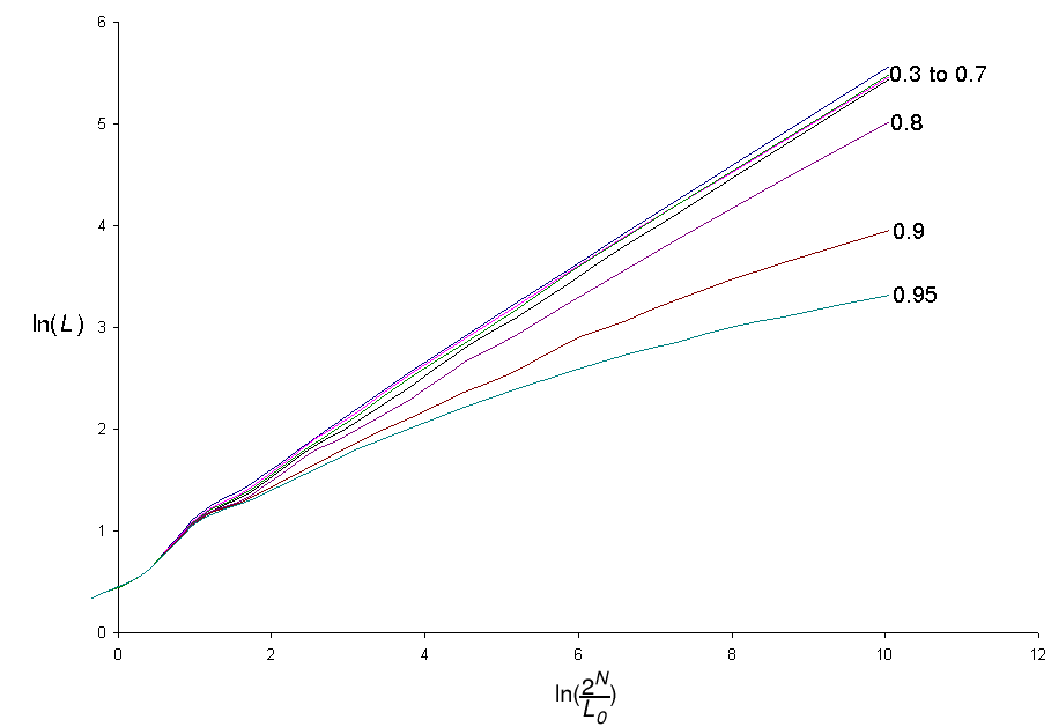
\includegraphics{Pix/frac-dims}}
  \parbox{110mm}{\caption{\label{fd} The length of the curve as a
    power law.  The top characteristics are virtually
    indistinguishable and correspond to the conditions in Figure
    \ref{new_f1} with reduction factors of the exclusion radius of
    0.3, 0.5, 0.6 and 0.7.  The remaining characteristics have the
    reduction factors indicated at their ends.}}
\end{center}
\end{figure}

Figure \ref{fd} shows plots of $\ln (L)$ against $\ln
(\frac{2^N}{L_0})$ for a range of radius reduction factors with the
conditions otherwise as in Figure \ref{new_f1}.  The data points have
been omitted for clarity, but are equally-spaced along the abscissa
for each characteristic and correspond to each value of $N$ from 0 to
15.  $L_0$, in this case, is $\sqrt 2$.

For reduction factors of 0.7 and below, the characteristics are
straight and virtually indistinguishable.  

It is clear that the line for a reduction factor of 0.95 is not
straight, though it is not clear whether its asymptote would be
finite.  A finite asymptote would imply that, even after infinite
recursion, the corresponding curve would still have a finite length.
A non-straight characteristic with an infinite value after infinite
recursion would imply a curve of infinite length, but not a curve that
was a scale-free self-similar fractal.  For scale-free self-similarity
the characteristic line has to be straight, like those for reduction
factors of 0.7 and below.

If each characteristic for reduction factors of 0.7 and below is
subjected to linear regression the average of the gradients, $d$, of
the resulting straight lines is 0.496 with a standard error of 0.002.
This means that for those four characteristics the mean fractal
dimension is 1.496, which---with the necessary caveats about small
sample size---tempts me to the intriguing conjecture that the true
value may be exactly 1.5.

\section*{Extending the idea}

\begin{figure}[h!]
 \begin{center} 
  \resizebox{0.4 \textwidth}{!}{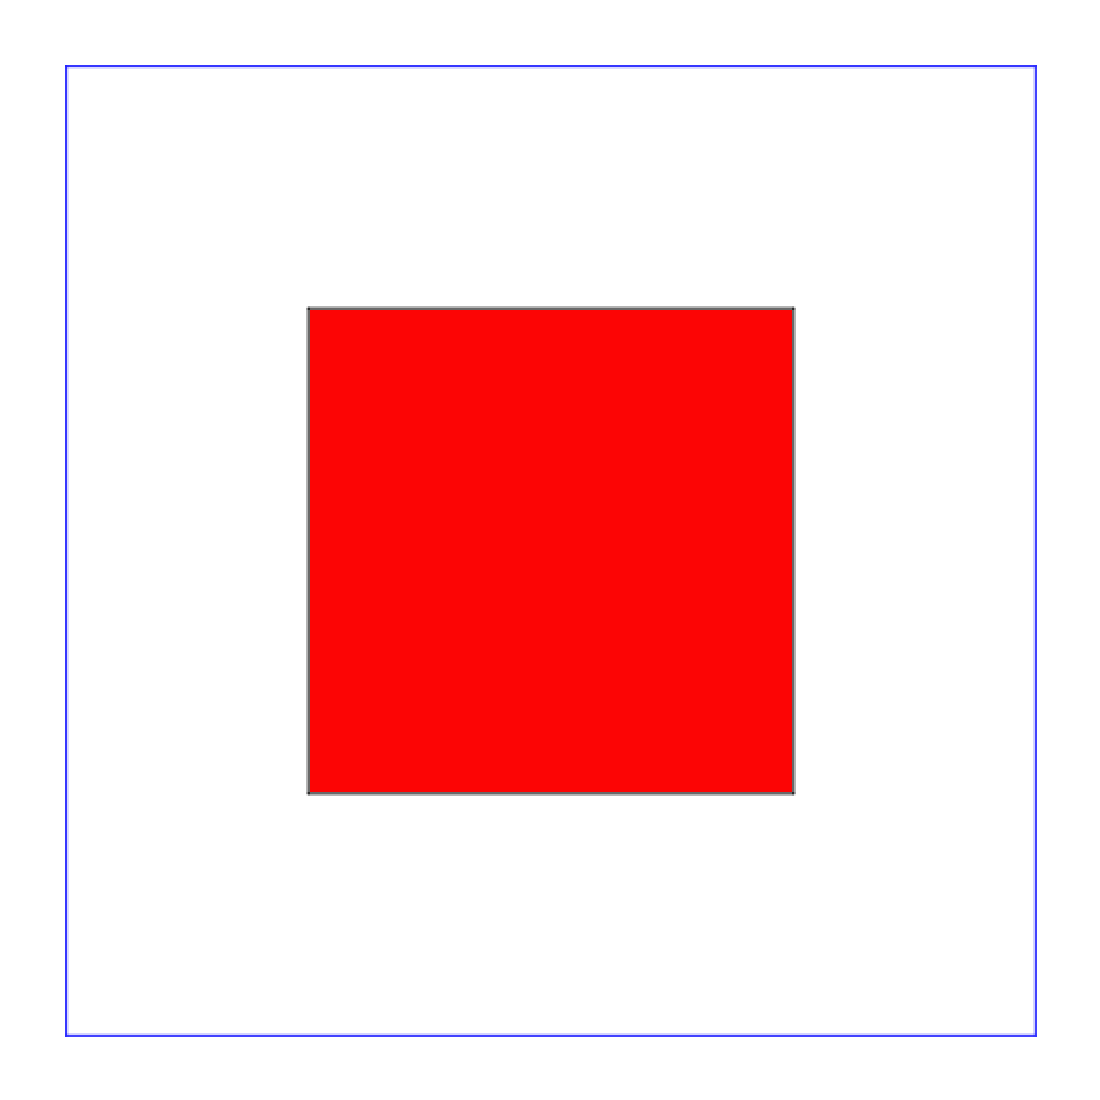
\includegraphics{Pix/loop0}}
  \resizebox{0.4 \textwidth}{!}{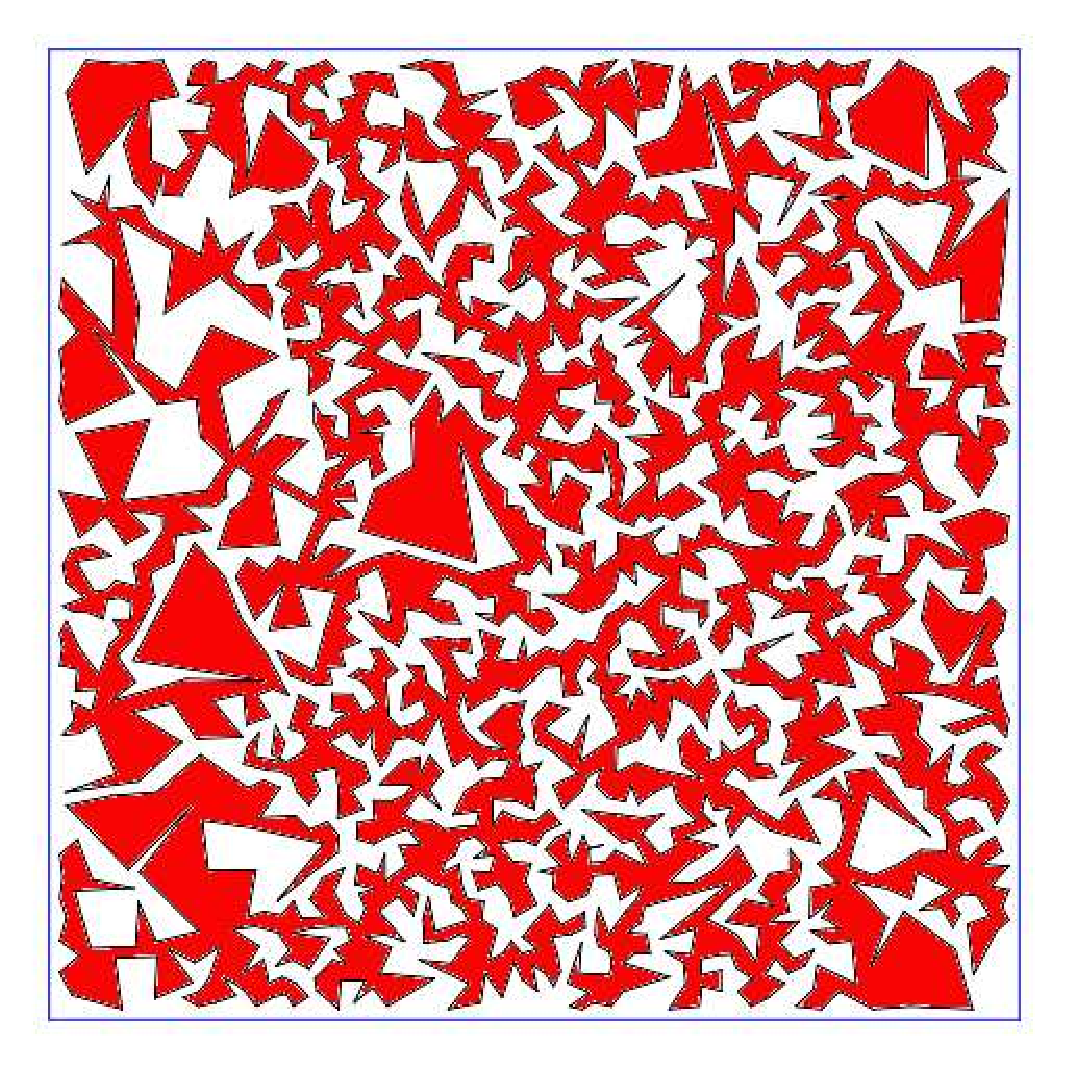
\includegraphics{Pix/loop}}
  \parbox{110mm}{\caption{\label{loop} A curve that started as a square of half the
  side-length of the bounding box placed at the box's centre.  The
  flood fill is to make the curve-generating method's preservation of
  the interior and the exterior clearer.}}
\end{center}
\end{figure}

Instead of starting with a single line segment, one can start with a
pre-defined polyline (or polygon, as with the triangle in Figure \ref{triang}).  Figure
\ref{loop} shows the result of starting with a square of side-length
0.5 in the middle of the unit bounding box.  The resulting closed
curve has been flood-filled to make the curve-generating-method's
preservation of the interior and the exterior clearer.

\begin{figure}[h!]
 \begin{center} 
  \resizebox{0.4 \textwidth}{!}{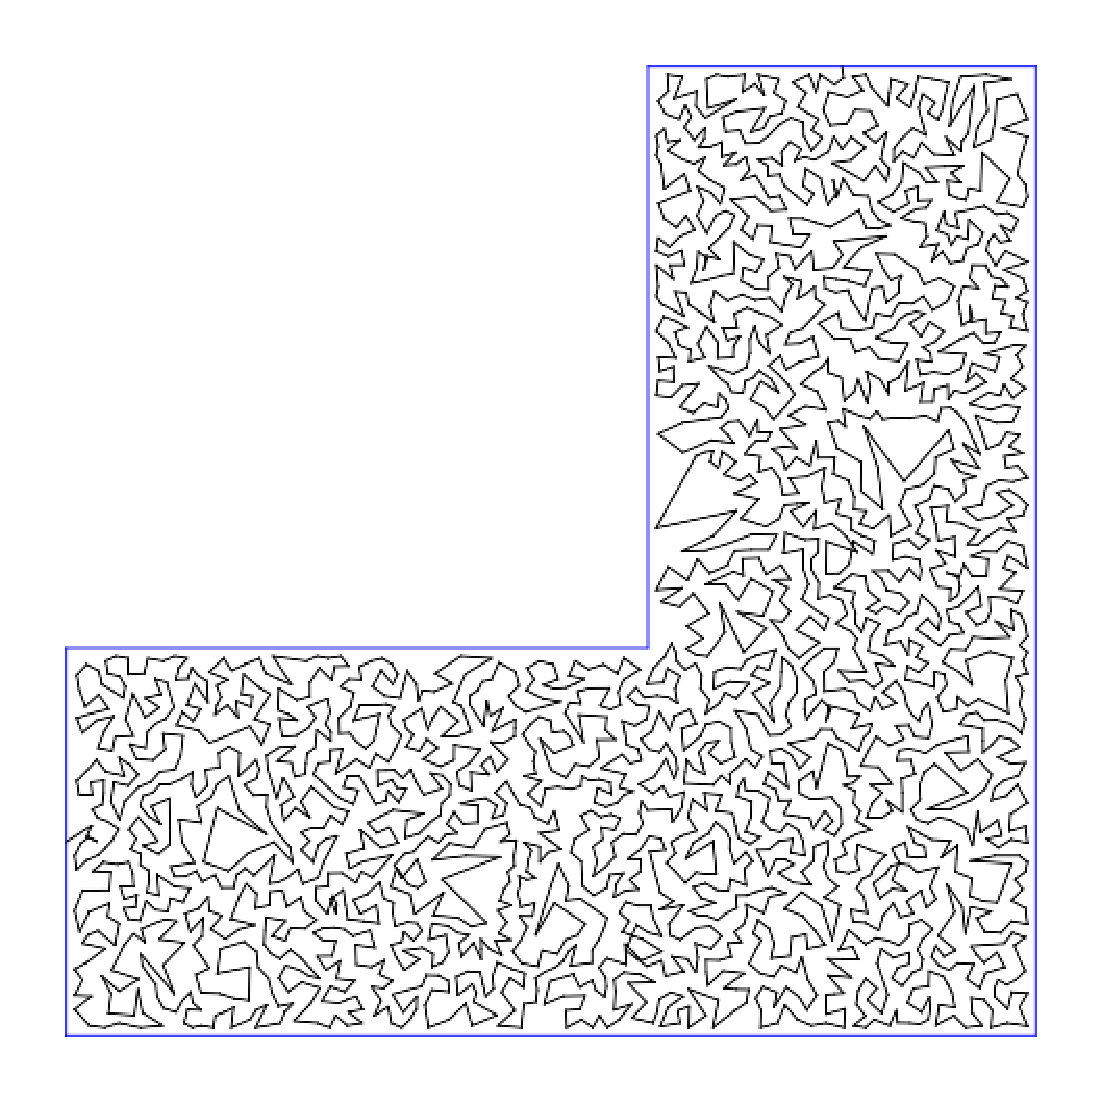
\includegraphics{Pix/bnd}}
  \parbox{110mm}{\caption{\label{bnd} The curve in an L-shaped bounding region; the
  starting curve was also L-shaped along the centre lines of the two
  limbs of the bounding region.}}
\end{center}
\end{figure}

The bounding region can be any shape.  Figure \ref{bnd} shows a curve
generated in an L-shaped bounding area.  This leads immediately to
the idea of running several intertwining curves at once.
\begin{figure}[h!]
 \begin{center} 
  \resizebox{0.4 \textwidth}{!}{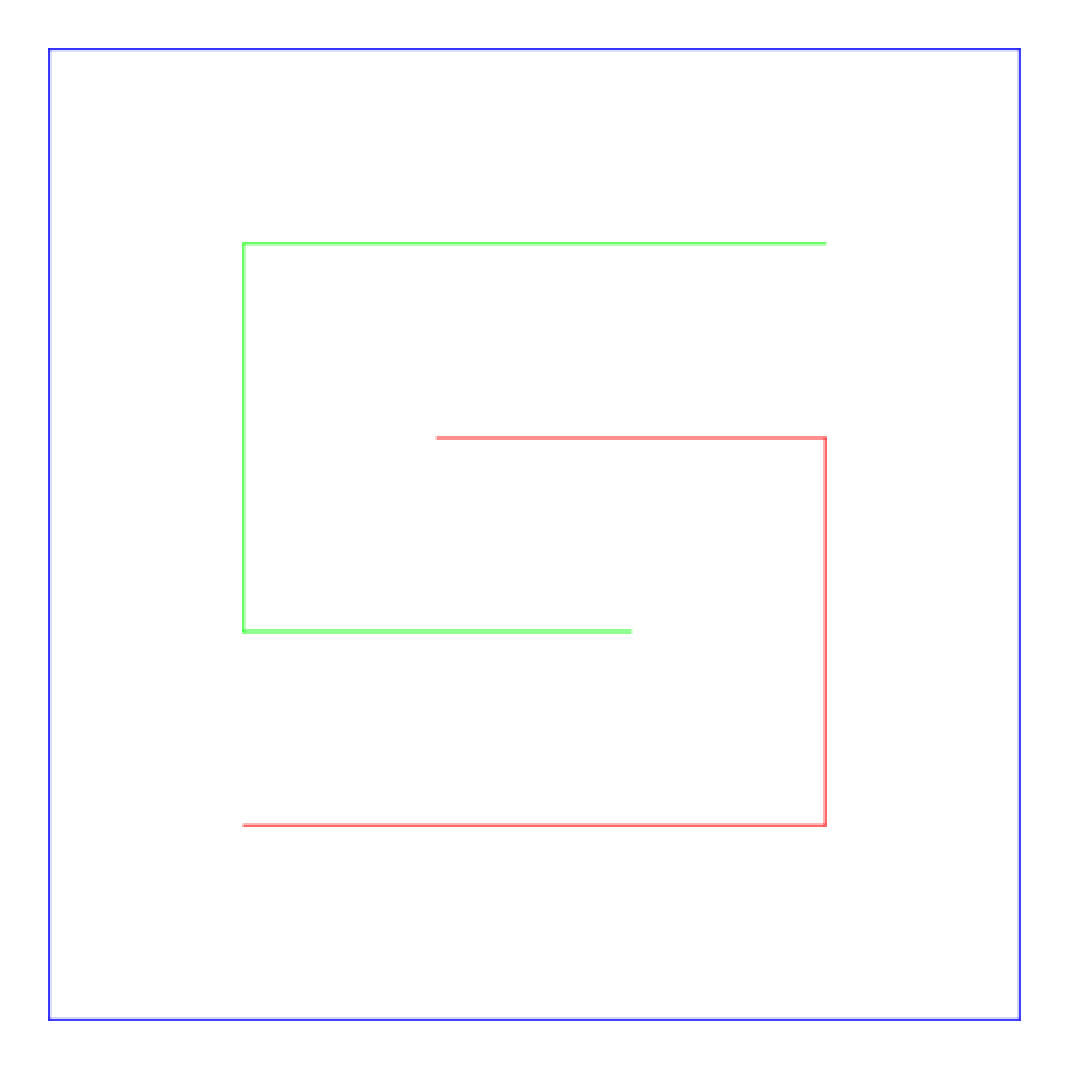
\includegraphics{Pix/ccstart}}
  \resizebox{0.4 \textwidth}{!}{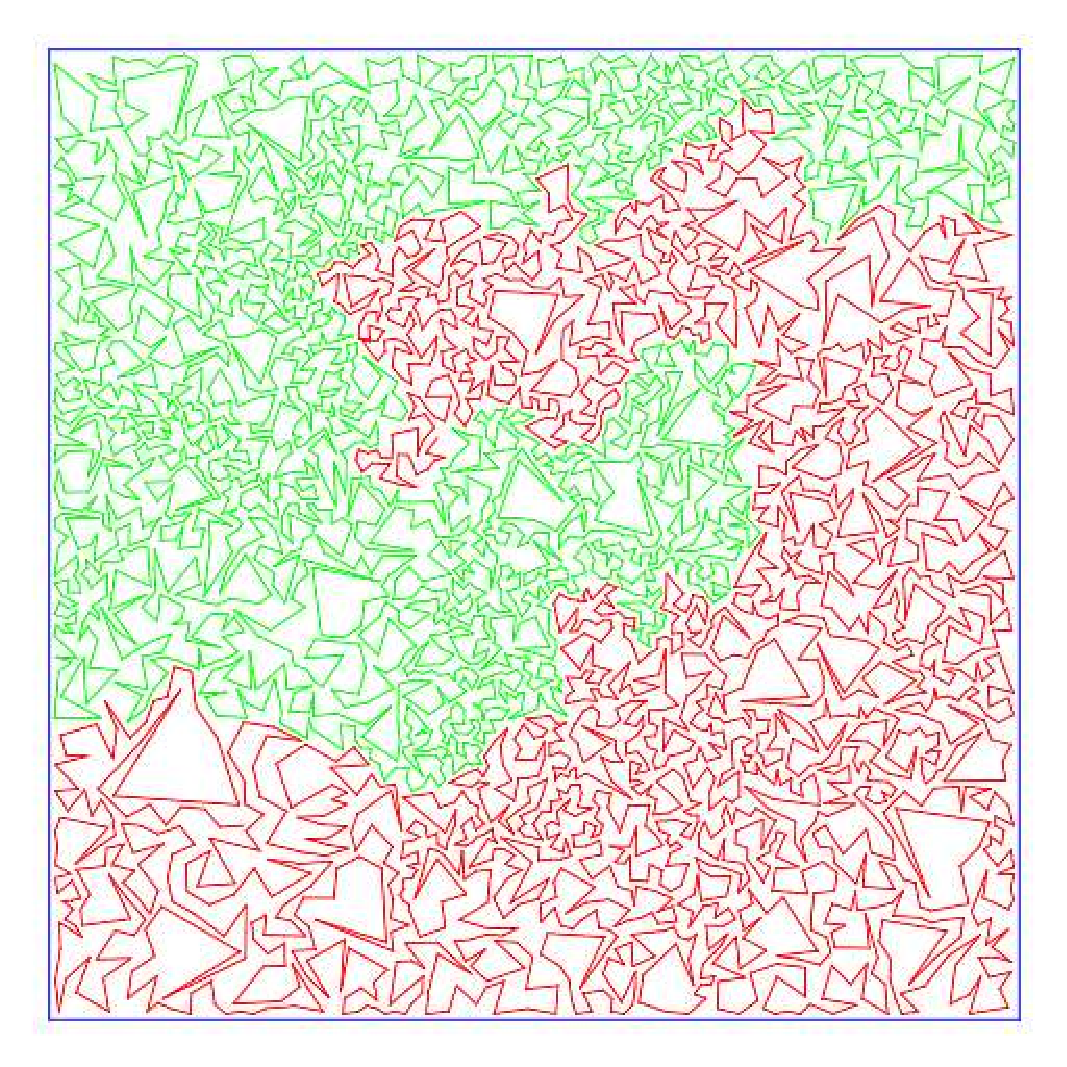
\includegraphics{Pix/cc}}
  \parbox{110mm}{\caption{\label{cc} The starting configuration, and
  the result of running the two starting polylines against each
  other.}}
\end{center}
\end{figure}
Figure \ref{cc} shows the
starting curves and the resulting curves from such an experiment.

\section*{Conclusions}

The curve that I needed would:

\begin{enumerate}

\item Fill any pre-defined closed connected area;

\item Be unbroken;

\item Not self-intersect;

\item Be possible to generate starting from any
given non-self-intersecting polyline within the area (including,
obviously, any single line segment);

\item Extend straightforwardly and comprehensively to any number of
 dimensions (especially 3); and

\item Be reasonably quick and simple to compute for finite recursions.

\end{enumerate}

\noindent
The curve presented in this report fulfils all those requirements.

Extending the curve in two-dimensions up to a surface in
three-dimensions is conceptually simple: the closed area would become
a closed volume (usually, though not necessarily, bounded by a
polyhedron) and the starting line segment (or segments) would become
triangle(s) within it.  There are a number of ways that a triangle can
be split into other triangles.  The simplest, perhaps, is to bisect
each edge and to join those points to form four new triangles.  (This
scheme is commonly used to generate random fractal landscapes, as
described by Hughes \cite{landscape}.)  The movement of the
splitting-points would be slightly more complicated than in two
dimensions: for splitting-points on edges that were interior to the
surface being created the points would be moved as far as possible
along a line that was perpendicular to the edge and that bisected the
dihedral angle between the two triangles that shared the edge; for
splitting points on edges at the boundary of the surface being created
the points would be moved as far as possible along a line that was
perpendicular to the edge and that lay in the plane of the triangle
owning the edge.  In both cases the points would be (as in two
dimensions) moved so that they and the triangles they defined came no
closer than the exclusion radius to anything else.  In $K$ dimensions
the triangles would become $K-1$ dimensional simplexes and the
boundary would usually (though again, not necessarily) be a polytope.

The next piece of work that I will do on this will be to write
software for constructing self-avoiding surfaces in three dimensions,
as just described.

\vspace{5mm}

\noindent
I would be most interested to hear of possible applications for the
new curve.  Also, as I intend to work on applications of it rather than
analysis of it myself, I would be interested to hear of analytical
results on its characteristics.  My e-mail address is given above.

\section*{Acknowledgement}

I would like to thank John Woodwark for his comments on the
first draft of this report.

\begin{thebibliography}{99}

\bibitem{texas-hilbert} V. B. Balayoghan (Department of Computer
Sciences, The University of Texas at Austin): applet for generating
various regular Peano curves at
http://www.cs.utexas.edu/users/vbb/misc/sfc/Oindex.html

\bibitem{boston-cps} Boston University
Center for Polymer Studies:  Coastline applet at
http://polymer.bu.edu/java/java/coastline/coastline.html

\bibitem{falconer} Kenneth Falconer: {\em Fractal Geometry:
Mathematical Foundations and Appications,} Wiley, ISBN 0 471 92287 0, 1990.

\bibitem{gpl} Free Software Foundation Inc.  (59 Temple Place - Suite
330, Boston, MA 02111-1307, USA): {\em GNU General Public License} at
http://www.gnu.org/copyleft/gpl.html

\bibitem{hilbert-orig} David Hilbert: {\em \"{U}ber die stetige Abbildung
einer Linie auf ein Fl\"{a}chenst\"{u}ck,} Math. Ann.,
{\bf 38}, pp. 459-460, 1891.

\bibitem{landscape}Merlin Hughes: {\em 3D Graphic Java: Render fractal
landscapes,} at
http://www.javaworld.com/javaworld/jw-08-1998/jw-08-step\_p.html

\bibitem{mandelbrot} Benoit B. Mandelbrot: {\em How Long is the Coast of
Great Britain: Statistical Self Similarity and Fractional Dimension,}
Science, {\bf 156}, 636-638, 1967.

\bibitem{mb2} Benoit B. Mandelbrot: {\em Fractals: Form, Chance, and
Dimension}, Freeman, ISBN 0716704730, 1977.

\bibitem{peano-orig} Giuseppe Peano: {\em Sur une courbe, qui remplit
toute une aire plane,} Math. Ann. {\bf 36}, pp. 157-160, 1890.

\bibitem{peitgen}Heinz-Otto Peitgen, Hartmut J\"{u}rgens, \& Dietmar
Saupe: {\em Chaos and Fractals -- New Frontiers of Science},
Springer-Verlag, ISBN 0-387-97903-4, 1992.

\bibitem{sagan} Hans Sagan: {\em Space-Filling Curves,} Springer-Verlag, New
York, ISBN 0-387-94265-3, 1991.

\end{thebibliography}




\end{document}
\grid
